\documentclass[10pt,a4paper]{article}
\usepackage[utf8]{inputenc}
\usepackage[french]{babel}
\usepackage{amsmath}
\usepackage{amsthm}
\usepackage{amsfonts}
\usepackage{amssymb}
\usepackage{graphicx}
\usepackage[a4paper,top=25mm,bottom=25mm]{geometry}
\author{Philipp Weder}
\title{Soutenance de stage - dispotition détaillée}





% packages for layout
\usepackage{fancyhdr}
\pagestyle{fancy}
\fancyhf{}
\fancyhead[L]{\textit{\nouppercase{\leftmark}}}
\fancyhead[R]{\thepage}

\renewcommand{\headrulewidth}{0.5pt}


%roman enumeration
\renewcommand\labelenumi{(\roman{enumi})}
\renewcommand\theenumi\labelenumi

% font
%\usepackage{pxfonts}

% bibliography
\usepackage[style=ieee, sorting = nty, backend = biber]{biblatex}
\bibliography{/Users/philipp/Documents/GitHub/stage_cmap/tex/Report/report.bib}
\usepackage{csquotes}

% environments
% theorem
\theoremstyle{plain}
\newtheorem{theorem}{Theorem}[section]
% corollary
\theoremstyle{plain}
\newtheorem{corollary}{Corollary}[theorem]
% lemma
\theoremstyle{plain}
\newtheorem{lemma}[theorem]{Lemma}
% remark
\theoremstyle{definition}
\newtheorem*{remark}{Remark}
% definition
\theoremstyle{definition}
\newtheorem{definition}{Definition}[section]
% example
\theoremstyle{definition}
\newtheorem{example}{Example}[section]
% proposition
\theoremstyle{plain}
\newtheorem{proposition}{Proposition}[section]

% additional packages
\usepackage{appendix}
\usepackage{amsmath}
\usepackage{amsfonts}
\usepackage{amssymb}
\usepackage{amsthm}
\usepackage{booktabs}

\newcommand{\N}{\mathbb{N}}
\newcommand{\M}{\mathcal{M}}
\newcommand{\R}{\mathbb{R}}
\newcommand{\h}{\mathcal{H}}
\newcommand{\K}{\mathcal{K}}
\DeclareMathOperator{\Skew}{Skew}
\DeclareMathOperator{\id}{id}
\newcommand{\so}{\mathfrak{so}}
\newcommand{\REF}{\mathrm{ref}}
\newcommand{\spr}{\textsc{SPr4}}
\DeclareMathOperator{\dist}{dist}
\DeclareMathOperator{\SO}{SO}
\DeclareMathOperator{\sgn}{sgn}
\DeclareMathOperator{\Aut}{Aut}
\DeclareMathOperator{\diag}{diag}
\newcommand{\chroexp}{\overset{\longrightarrow}{\exp}}
\DeclareMathOperator{\re}{Re}
\DeclareMathOperator{\Span}{span}
\newcommand{\dd}[1]{\mathrm{d}#1}
\DeclareMathOperator{\ad}{ad}
\newcommand{\T}{\mathcal{T}}

\begin{document}
\renewcommand\labelitemi{--}
\linespread{1.1}
\maketitle
\section{Mot de bienvenue}
\begin{itemize}
\item Bonjour à tous....
\item Pendant mon stage, je me suis occupé du sujet de la \emph{natation à l'échelle microscopique}. Plus précisement, j'ai analysé un micro-nageur, qu'on a appelé "parking 4-sphere swimmer"(\textsc{SPr4}) que je vais vous présenter tout de suite. Mais commençons par le début...
\end{itemize}
\section{Introduction}
\begin{itemize}
\item Edward Purcell était le premier à publier ses idées sur la natation à l'échelle microscopique en 1977 dans son papier "Life at low Reynolds number" \cite{Purcell1977}. En particulier, il a démontré le fameux "scallop theorem" qui dit qu'une coquille Saint Jacques microscopique ne peut pas nager.

\item Cette observation a motivé la recherche pour le mécanisme le plus simple de natation à l'échelle microscopique. Jusque là, des nombreux tels mécanismes ont été analysés, au moins partiellement. Voici, trois exemple: Le nageur \textsc{3S} à gauche qui ne peut se déplacer sur une droite, le nageur \textsc{SPr3} dont on sait de \cite{Alouges2017} qu'il peut se déplacer dans un plan et puis le nageur \textsc{SPr4} qui a été traité dans ce projet.

\item Le problème mathématique principal est qu'à l'échelle microscopique le nombre de Reynolds $\re = \rho u L/\mu$ est très bas, ce qui entraîne que dans les équations de Navier-Stokes les forces d'inertie deviennent négligeables. Par conséquent, un micro-nageur ne peut utiliser que les forces visqueuses pour se déplacer. Plus précisément, un micro-nageur est régit par les équations de Stokes qui sont linéaires et réversibles par rapport au temps. Ceci implique en particulier qu'un mouvement réciproque ne contribuera pas au déplacement!

\item En termes mathématiques, on face on problème de contrôlabilité, c'est-à-dire on veut trouver un mécanisme pour nager avec un nombre le plus petit possible de contrôles tel que l'on puisse atteindre n'importe quelle position dans l'espace avec une suite de mouvements périodiques.

\item Une question supplémentaire naturelle est celle de la natation optimale, c'est-à-dire trouver les mouvements optimaux par rapport à la consommation d'énergie.

\item Pour le nageur \textsc{SPr4}, le problème de contrôlabilité a déjà été résolu dans \cite{Alouges2013}. Or, on n'a pas encore des expressions explicites.

\item Dans mon projet, j'ai analysé le nageur \textsc{SPr4} analytiquement sous l'hypothèse que les mouvements soient petits. Ensuite, j'ai essayé sous la même hypothèse de trouver la structure des courbes de contrôle optimales. Portant, je n'y suis parvenu que pour une classe particulière de déplacements prescrits. Bien sûr, on a également exploré le cas général.
\end{itemize}


\section{Structure du projet}
La structure du reste de la présentation est comme ce qui suit:
\begin{enumerate}
\item Tout d'abord, je vais vous présenter le modèle mathématique qui a été introduit dans \cite{Alouges2013} et je vais vous montrer les propriétés de symétrie satisfaites par le système de contrôle en question.

\item Ensuite, je vais introduire l'hypothèse des courbes de contrôle petites et je vais présenter les implications qui en résultent pour notre système de contrôle. 

\item Puis, je parlerai du problème d'optimisation associé dont on verra la solution dans un cas particulier.

\item Finalement, j'aborderai les perspectives sur le sujet et je présenterai la conjecture sur le cas général, qu'on a faite à la fin du projet.
\end{enumerate}


\section{Modélisation et symétries}
\subsection{Notation et modèle}
\begin{itemize}

\item Pour le modèle du nageur vu avant, on se donne un tétraèdre de référence avec sommets $(S_1, S_2, S_3, S_4)$ centré à $c \in \R^4$ tel que $\dist(c, S_i) = 1$.

\item Alors le nageur \textsc{SPr4} consiste de quatre boules $B_i$ centrées à $b_i$ de rayon $a > 0$ telles que la boule $B_i$ peut bouger le long de la demi-droite d'origine $c$ passant par $S_i$.

\item Donc, on est dans la situation où les quatre boules sont reliées à $c$ par des bras très fin, qui peuvent s'allonger et se rétracter. Or, on néglige la résistance visqueuse des bras. De plus, il n'y a aucune restriction pour l'orientation du nageur dans le fluide, c'est-à-dire à longueurs de bras fixés, le nageur est juste un corps rigide dans un fluide Stokesien.

\item La configuration géométrique est complètement décrite par deux ensembles de variables:
\begin{enumerate}
\item \emph{Les variables de forme:} $\xi := (\xi_1, \xi_2, \xi_3, \xi_4) \in \M := (\sqrt{3/2}a, + \infty)^4$, où les $\xi_i$ sont les longueurs des bras.

\item \emph{Les variables de position:} $p = (c, R) \in \mathcal{P} := \R^3 \times \SO(3)$.
\end{enumerate}
De plus, on pose $z_i := \overline{S_i c}$. 

\item Dans \cite{Alouges2013}, il a été montré comment $p$ change si on varie $\xi$. Plus précisément, on a le système dynamique suivant:
\begin{equation}
\label{eq: control system}
	\dot{p} = F(R, \xi) \dot{\xi} := \left ( \begin{array}{c}
	F_c(R, \xi) \\
	F_\theta(R, \xi)
	\end{array}  \right ) \dot{\xi},
\end{equation}
tel que $\dot{c} = F_{c}(R, \xi) \dot{\xi}$ et $\dot{R} = R_{\theta}(R, \xi) \dot{\xi}$.

\item On remarque qu'on a
\begin{equation}
\begin{aligned}
	F_c(R, \xi) \in \mathcal{L}(\R^4, \R^3) \text{ et } F_{\theta}(R, \xi) \in \mathcal{L}(\R^4,T_R \SO(3)).
\end{aligned}
\end{equation}
Donc, dès qu'on a fixé des bases, on peut les exprimer comme des matrices de taille $3 \times 4$.

\end{itemize}

\subsection{Symétries}
%Passons à l'investigation du système de contrôle \ref{eq: control system}. Pour ceci, choisissons une condition initiale $p_0 = (c_0, R_0) \in \mathcal{P}$ et une courbe de contrôle $\xi: J \subset \R \to \M$, avec $J$ un voisinage de zéro. Puis, notons $\gamma(c_0, R_0, \xi): I \to \mathcal{P}$ la solution associée au système dynamique
%\begin{equation}
%\label{eq:dynamical system}
%\begin{aligned}
%	&\dot{p} = F(R, \xi) \dot{\xi},& & p(0) := p_0.
%\end{aligned}
%\end{equation}
%On notera par $\gamma_c(c_0, R_0, \xi)$ et $\gamma_{\theta}(c_0, R_0, \xi)$ les projections à $\R^3$ et $\SO(3)$, respectivement. En particulier, on a par définition
%\begin{equation}
%	\dot{\gamma}(c_0, R_0, \xi)(t) = F(\gamma_\theta(c_0, R_0, \xi)(t), \xi(t))\dot{\xi}(t), \forall t \in J.
%\end{equation}

\begin{itemize}
\item Passons à l'investigation du système de contrôle (\ref{eq: control system}) sur la base des symétries satisfaites par les équations de Stokes.

\item Notamment, les équations de Stokes sont invariantes sous rotations et sous changement de point de vue.

\item Donc, on a appliqué les transformations correspondantes à une solution du système dynamique et puis on a déterminée comment $F$ se transforme par différentiation. 
\end{itemize}

\subsubsection{Invariance rotationelle}
%\begin{itemize}
%
%\item Les équations de Stokes sont invariant sous rotations, c'est-à-dire si on tourne tout le domaine géométrique, la solution se transforme de la même façon.
%
%\item Ceci implique pour la solution de notre système dynamique que
%\begin{equation}
%\label{eq:spatial rotational invariance}
%	\gamma_c(c_0, R R_0, \xi)(t) = R \gamma_c (c_0, R_0, \xi)(t) + (I - R) c_0, \forall t \in J
%\end{equation}
%et
%\begin{equation}
%\label{eq: angular rotational invariance}
%	\gamma_\theta(c_0, R R_0, \xi)(t) =  R \gamma_\theta(c_0, R_0, \xi)(t), \forall t \in J
%\end{equation}
%Ensuite, on trouve avec un calcul la propriété suivante du champs de vecteur $F$:
%\begin{eqnarray}
%	F_c(R, \xi) = R F_c(\xi) \text { and } F_\theta(R, \xi) = R F_{\theta} (R, \xi),&  \forall (R, \xi) \in \SO(3) \times \M,
%\end{eqnarray}
%où $F_c(\xi) := F_{c}(I, \xi)$ et $F_{\theta}(\xi) := F_{\theta}(I, \xi)$.
%
%\item Ceci signifie juste qu'on peut toujours factoriser l'orientation de $F$.
%
%\end{itemize}

De l'invariance rotationnelle des équations de Stokes, on déduit que pour toute rotation $R \in \SO(3)$, on a
\begin{eqnarray}
	F_c(R, \xi) = R F_c(\xi) \text { and } F_\theta(R, \xi) = R F_{\theta} (R, \xi),&  \forall (R, \xi) \in \SO(3) \times \M,
\end{eqnarray}
où $F_c(\xi) := F_{c}(I, \xi)$ et $F_{\theta}(\xi) := F_{\theta}(I, \xi)$.


\subsubsection{Permutation des bras}
\begin{itemize}
\item On veut profiter de l'invariance des équations de Stokes sous changement de point de vue pour déterminer comment $F$ se transforme lors d'une permutations de deux bras.

\item Notons $P_{ij} \in M{4 \times 4}(\R)$ la matrice de permutation qui échange les indices $i$ et $j$ d'un vecteur. Cette transformation appliquée à l'espace de contrôles $\M$ signifie la permutation des bras $i||$ et $j||$.

\item Soit $S_{ij}$ la réflexion qui envoie $i ||$ sur $j||$ dans $\mathcal{P}$. 

%\item Les équations sont invariantes sous changement de point de vue, ce qui implique pour notre solution que pour la position initiale $p_0 := (c, I)$ on a
%\begin{equation}
%\label{eq:spatial_perm_inv}
%	\gamma_c(c_0, I, P_{ij} \xi) = S_{ij} \gamma_c(S_{ij}c_0, I, \xi)
%\end{equation}
%et
%\begin{equation}
%\label{eq:angular_perm_inv}
%	\gamma_{\theta}(c_0, I, P_{ij} \xi ) = S_{ij} \gamma_{\theta} (S_{ij} c_0, I, \xi) S_{ij}.
%\end{equation}

\item En effet, la permutation des bras $||i$ et$||j$ correspond à regarder la trajectoire dans un miroir qui envoie le bras $||i$ sur $||j$, i.e. qui correspond à $S_{ij}$. Ainsi, on peut exploiter l'invariance des équations de Stokes.

\item À l'aide d'un calcul un peu plus technique, on trouve le résultat suivant:
\begin{align}
	 F_c(P_{ij} \xi) = S_{ij} F_c(\xi) P_{ij} \text{ et } F_{\theta}(P_{ij} \xi) = - S_{ij} F_{\theta}(\xi) P_{ij}. \forall \xi \in \M.
\end{align}


\item Attention: Il faut toujours choisir la base canonique $\mathcal{E} = (e_1, e_2,e_3, e_4$ pour $\R^4$ et la base $\mathcal{L} = (L_1, L_2, L_3)$ avec
\begin{align}
\label{eq: L1}
	&L_1 = \left(\begin{array}{ccc}
	0 & 0 & 0 \\ 
	0 & 0 & -1 \\ 
	0 & 1 & 0
	\end{array}  \right ),\\
\label{eq: L2}
	&L_2  = \left (\begin{array}{ccc}
	0 & 0 & 1 \\ 
	0 & 0 & 0 \\ 
	-1 & 0 & 0
	\end{array}  \right ),\\
\label{eq: L3}
	&L_3  = \left (\begin{array}{ccc}
	0 & -1 & 0 \\ 
	1 & 0 & 0 \\ 
	0 & 0 & 0
	\end{array}  \right ),
\end{align}
pour justifier la notation dans l'équation à droite dans la proposition.
\end{itemize}

\section{Régime des petites courbes de contrôle}
\begin{itemize}
\item Maintenant, on a envie d'exploiter les propriétés de symétrie de $F$ de la partie précédente. Pour faire ceci, attaquons $F$ du côté analytique. 

\item On part de la factorisation
\begin{equation}
\label{eq: reminder control system}
	F_{c}(R, \zeta) = R F_{c}(\zeta) \text{ et } F_{\theta}(R, \xi) = R F_{\theta}(\zeta), \forall R \in \SO(3),
\end{equation}
où $F_{c}(\zeta) := F_c(I, \zeta)$ et $F_{\theta}(\zeta) := F_{\theta}(I, \zeta)$. Puis, supposons que $\zeta = \xi_0 + \xi$, où $\xi_0$ a toutes les composoantes égales. Finalement, posons $F_{c, \xi_0}(\xi) := F_{c}(\xi_0 + \xi)$ et $F_{\theta, \xi_0}(\xi) := F_{\theta}(\xi_0 + \xi)$.

\item Il a été démontré dans \cite{Alouges2013} que $F$ et donc $F_{c, \xi_0}$ et $F_{\theta, \xi_0}$ sont analytiques. Par conséquents, nous avons le droit de faire le développement limité suivant:
\begin{align}
\label{eq: spatial control expansion}
	F_{c, \xi_0}(\xi)\eta &= F_{c, 0} \eta  + \h_{c,0}(\xi \otimes \eta) + \mathcal{O}(|\xi|)\eta\\
\label{eq: angular control expansion}
	F_{\theta, \xi_0}(\xi) \eta &= F_{\theta, 0} \eta + \h_{c, 0}(\xi \otimes \eta) + \mathcal{O}(|\xi|)\eta,
\end{align}
où $F_{c,0} := F_{c}(\xi_0) \in M_{3 \times 4}(\R)$, $\h_{c,0}\in \mathcal{L}(\R^4 \otimes \R^4, \R^3)$ représent la dérivée d'ordre 1 de $F_{c, \xi_0}$ à $\xi = 0$. $F_{\theta, \xi}$ est défini de façon analogue.

\item Pour les termes d'ordre zéro on peut montrer que
\begin{align}
\label{eq:zeroth_order_sym}
	F_{c,0} &= S_{ij} F_{c,0} P_{ij}\\
	F_{\theta, 0} &= -S_{ij} F_{\theta, 0} P_{ij}
\end{align}
ainsi que pour les termes d'ordre un que
\begin{align}
\label{eq:first_order_sym}
\h_{c,0}(P_{ij} \xi\otimes \eta) &= S_{ij} \h_{c,0}(\xi \otimes P_{ij} \eta), &\forall \xi, \eta \in \R^4\\
\h_{\theta,0}(P_{ij} \xi \otimes \eta) &= -S_{ij} \h_{\theta,0}(\xi \otimes P_{ij} \eta), &\forall \xi, \eta \in \R^4
\end{align}

\item Donc, on dispose de deux grands systèmes d'équations vectorielles, dont on veut déterminer l'espace de solutions.
\end{itemize}

\subsection{Termes d'ordre zéro}
\begin{itemize}
\item Un calcul élémentaire, qui n'utilise que (\ref{eq:zeroth_order_sym}) et les propriétés des $S_{ij}$ montre que
\begin{equation}
	F_{c,0} = \mathfrak{a} (z_1 |z_2| z_3|z_4),
\end{equation}
avec $\mathfrak{a} \in \R$ ou bien
\begin{equation}
	F_{c,0} = - 3 \sqrt{3} \mathfrak{a} [\tau_1| \tau_2 |\tau_3]^T,
\end{equation}
où $\tau_1 : = \tfrac{1}{\sqrt{6}}(-2,1,1,0)^T$, $\tau_2 := \tfrac{1}{\sqrt{2}}(0,1,-1,0)^T$, $\tau_{3}:= \tfrac{1}{2 \sqrt{3}} (1,1,1,-3)^T$ forment une base orthonormale ensemble avec $\tau_4:= \tfrac{1}{2}(1,1,1,1)^T$. Cette base orthonormale sera utile plus tard.
\end{itemize}

\subsection{Termes d'ordre un}
\begin{itemize}
\item Pour déterminer les termes d'ordre un, on a suivi l'approche dans \cite{Alouges2017}, où on a évalué les tenseurs sur la base canonique et où on a posé
\begin{align}
A_k &:= (\h_{c,0}(e_i \otimes e_j)\cdot \hat{e}_k)_{i,j \in \N_4}, k \in \N_3\\
B_k &:= (\h_{\theta,0}(e_i \otimes e_j)\cdot \hat{e}_k)_{i,j \in \N_4}, k \in \N_3.
\end{align}
Ainsi, on a pour tout $\xi, \eta \in \R^4$
\begin{align}
\label{eq: matrix representation of spatial first order term}
	\h_{c,0}(\xi \otimes \eta) = \sum_{k \in \N_3}(A_k \eta \cdot \xi)\hat{e}_k, \\
\label{eq: matrix representation of angular first order term}
	\h_{\theta, 0}(\xi \otimes \eta) = \sum_{k \in \N_3}(B_k \eta \cdot \xi) L_k.
\end{align}

\item À lieu de calculer directement les matrices $A_k$ et $B_k$, on a calculé leurs parties symétriques et anti-symétriques en utilisant des arguments de symétrie. En fait, seulement les parties anti-symétriques seront importantes pour la suite. Notons-les
\begin{align}
M_k &:= \frac{1}{2}[A_k - A_k^T], k \in \N_3\\
M_{k + 3} &:= \frac{1}{2}[B_k - B_k^T], k \in \N_3.
\end{align}

\item Finalement, il ne reste que 5 paramètres inconnus dans les matrices $A_k$ et $B_k$.
\end{itemize}

\subsection{Linéarisation}
\begin{itemize}
\item Maintenant, on se donne un espace pour les courbes, notamment $H^1_{\sharp}(J, \R^4)$, où $J := [0, 2\pi]$.

\item On notera $\langle f \rangle := (2 \pi)^{-1 }\int_{J} f(t) d t$ pour $f \in H^1_{\sharp}(J, \R^4)$ la moyenne d'une fonction.

Puis dans la partie précédente, on a posé $\zeta = \xi_0 + \xi$ et un développement limité autour de $\xi = 0$ nous a fournit le système simplifié
 \begin{align}
 \label{eq: dynamics first approx}
 \begin{cases}
 	\dot{c} &= R F_{c,0} \dot{\xi} + R \sum_{k \in \N_3}(A_k \dot{\xi} \cdot \xi)\hat{e_k}\\
 	\dot{R} &= R \sum_{k \in \N_3} (B_k \dot{\xi} \cdot \xi) L_k.
 \end{cases}
 \end{align}
 
\item Définissons les déplacements nets
\begin{align}
	\delta c: &H_{\sharp}^1(J,\R^4) \to \R^3, &
	\delta p: & H_{\sharp}^1(J,\R^4) \to \so(3)\\
	&\xi \mapsto 2\pi \langle \dot{c} (\xi) \rangle \nonumber, &
	&\xi \mapsto 2 \pi \langle \dot{R}(\xi) \rangle \nonumber
\end{align}
Il est impossible d'évaluer ses expressions exactement, mais un argument du calcul chronologique nous a permis de linéariser le système simplifié autour de $R_0 = I$. Ainsi, on est arrivé à établir le résultat suivant:
\begin{proposition}
\label{prop:net displacement}
Pour tout $\xi \in H_\sharp^1(J, \R^4)$, dans un voisinage de $0 \in H_{\sharp}^{1}(J, \R^4)$, on a les estimes suivants
\begin{equation}
\begin{aligned}
\delta c(\xi) &= 2 \pi \sum_{k \in \N_3} \langle A_k \dot{\xi} \cdot \xi \rangle \hat{e}_k + \mathcal{O}(||\xi||_{H^1_{\sharp}}^3),\\
\delta R(\xi) &= 2 \pi \sum_{k \in \N_3} \langle B_k \dot{\xi} \cdot \xi \rangle L_k + \mathcal{O}(||\xi||^4_{H_\sharp^1}).
\end{aligned}
\end{equation}
\end{proposition}

\item Si $A$ est une matrice symétrique, on trouve par intégration par parties que $\langle A \xi \cdot \dot{\xi} \rangle = - \langle A \xi \cdot \dot{\xi} \rangle = 0$ et donc
\begin{align}
\langle A_k \dot{\xi} \cdot \xi \rangle &= \langle M_k \dot{\xi} \cdot \xi \rangle, &\forall k \in \N_3\\
\langle B_k \dot{\xi} \cdot \xi \rangle &= \langle M_{k + 3} \dot{\xi} \cdot \xi \rangle, &\forall k \in \N_3
\end{align}

\item Si on note $\{f_k\}_{k \in \N_6}$ la base canonique de $\R^6$, un calcul montre que
\begin{equation}
\label{eq: net displacement}
\frac{\delta p}{2 \pi}= - 2  \sqrt{6} \alpha \sum_{k \in \N_3}\langle \det( \xi | \dot{\xi} | \tau_{k+1} | \tau_{k+2})\rangle f_k  - 2  \sqrt{6} \delta \sum_{k \in \N_3}\langle \det ( \xi | \dot{\xi} | \tau_{k} | \tau_{4})\rangle f_{k + 3},
\end{equation}
où $k$ pris mod 3.

\item En résumé, jusque là on a établit la dynamique du nageur dans le régime de petites courbes de contrôle à cinq paramètres près et on sait exprimer le déplacement net à 3 paramètres près.
\end{itemize}

\section{Optimisation I}
\begin{itemize}
\item On adopte la définition d'efficacité selon Lighthill \cite{Lighthill1952}: Les mouvements optimaux sont ceux qui minimisent la dissipation d'énergie cinétique en atteignant un déplacement net prescrit.

\item En termes mathématiques, la dissipation d'énergie due à un mouvement $\xi \in H^1_{\sharp}(J, \R^4)$ s'écrit par une fonctionnelle d'énergie appropriée
\begin{equation}
 \mathcal{G}(\xi) := \int_{J} \mathfrak{g}(\xi(t))\dot{\xi}(t) \cdot \dot{\xi}(t) \dd t,
\end{equation}
où la densité d'énergie $\mathfrak{g} \in C^1(\R^4)$ est une fonction à valeurs dans les matrices symétriques et définies positives de $M_{4 \times 4}(\R)$. (En fait, c'est une métrique Riemannienne)

\item Sous l'hypothèse des petites courbes de contrôle, on peut supposer que $\mathfrak{g}(\xi) = \mathfrak{g}(0) + o(1)$, avec $\mathfrak{g}(0)$ une matrice symétrique définie positive dans $M_{4 \times 4}(\R)$. Ainsi, l'énergie s'écrit
\begin{equation}
\label{eq: linearized energy functional}
	\mathcal{G}(\xi) := \int_{J} Q_{\mathfrak{g}}(\dot{\xi}(t))\dd t,
\end{equation}
avec $Q_{\mathfrak{g}}$ la forme quadratique associée à la matrice $\mathfrak{g}(0)$, i.e. $Q_{\mathfrak{g}}(\eta) := \mathfrak{g}(0)\eta \cdot \eta$.

\item Les propriétés de symétrie des équations Stokes impliquent en particulier que
\begin{align}
	Q_{\mathfrak{g}}(P_{ij} \eta) = Q_{\mathfrak{g}}(\eta),\; i,j \in \N_4.
\end{align}
On en déduit avec un petit calcul que la matrice $G$ qui représente $Q_{\mathfrak{g}}$ est de la forme suivante:
\begin{equation}
G = \left ( \begin{array}{cccc}
\kappa & h & h & h \\ 
h & \kappa & h & h \\ 
h & h & \kappa & h \\ 
h & h & h & \kappa
\end{array} \right ),
\end{equation}
pour deux paramètres $h$ et $\kappa > \max(h, -3h)$. En particulier, on observe que $G \tau_k = (\kappa - h ) \tau_k$ pour $k \in  \N_3$ et $G \tau_4 = (\kappa + 3h) \tau_4$. Dans la suite on notera $\mathfrak{g}_1 := \mathfrak{g}_2 := \mathfrak{g}_3 := \kappa - h$ et $\mathfrak{g}_4 := \kappa + 3h$ les valeurs propres de $G$. Ensuite, on diagonalise $G$:
\begin{eqnarray}
G = U \Lambda_{\mathfrak{g}} U^T, & U := [\tau_1 | \tau_2 |\tau_3 |\tau_4], & \Lambda_{\mathfrak{g}} := \diag(\mathfrak{g}_i).
\end{eqnarray}

\item Donc, on face le problème d'optimisation suivant: Trouver $ \inf_{\xi \in H_{\sharp}^1(J, \R^4)} \int_{J} Q_{\mathfrak{g}}(\dot{\xi}(t)) \dd t$ sous la contrainte 
\begin{align}
\label{eq: constraint}
\delta p = \mathfrak{h}_{c} \sum_{k \in \N_3}\left ( \int_{J} \det( \xi(t) | \dot{\xi}(t) | \tau_{k+1} | \tau_{k+2}) \dd t \right ) f_k\\
	+ \mathfrak{h}_{\theta}  \sum_{k \in \N_3}\left ( \int_{J} \det ( \xi(t) | \dot{\xi}(t) | \tau_{k} | \tau_{4}) \dd t\right ) f_{k + 3} \nonumber,
\end{align}
	avec $\mathfrak{h}_c = - 2 \sqrt{6} \alpha$ et $\mathfrak{h}_{\theta} = - 2 \sqrt{6} \delta$.
\end{itemize}


\section{Bivecteurs en $\R^4$}
\begin{itemize}
\item Pour bien révéler la structure du problème ainsi que pour bien comprendre les différences entre le nageur \textsc{SPr3} de \cite{Alouges2017} et \textsc{SPr4}, on aura besoin de la notion de bivecteur.

\item Sans entrer dans les détails, je vais illustrer la notion sur la base du cas $\R^3$. Un bivecteur dans $\R^3$ est juste un petit parallélogramme avec magnitude donnée par la surface et la direction donnée par l'orientation du parallélogramme dans $\R^3$ ensemble avec l'orientation des vecteurs aux bords. De plus, on a envie de comprendre un bivecteur comme un produit des vecteurs aux bords, ce qui est exactement réalisé par le produit "wedge".

\begin{figure}[h]
\center
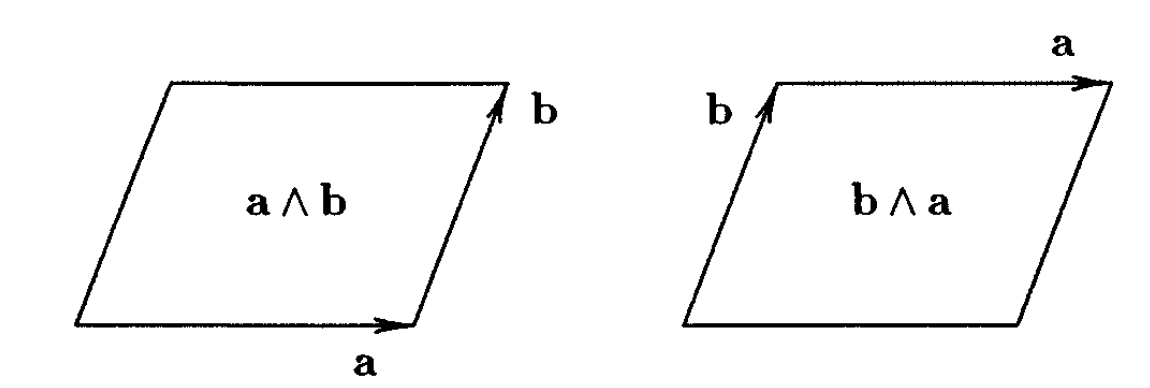
\includegraphics[scale=0.5]{/Users/philipp/Documents/GitHub/stage_cmap/tex/Présentation/images/bivecteurs.png}
\end{figure}

\item Ainsi, les bivecteurs forment un espace vectoriel $\bigwedge^2 \R^3$ avec une base donnée par
\begin{equation}
 \{\hat{e}_1 \wedge \hat{e}_2, \hat{e}_1 \wedge \hat{e}_3, \hat{e}_2 \wedge \hat{e}_3\},
\end{equation}
si $\{\hat{e}_1, \hat{e}_2, \hat{e}_3\}$ est une base de $\R^3$. En outre, le produit scalaire est donné par
\begin{equation}
( u_1 \wedge u_2 , v_1 \wedge v_2 ) = \det \left (\begin{array}{cc}
u_1 \cdot v_1 & u_1 \cdot v_2 \\ 
u_2 \cdot v_1 & u_2 \cdot v_2
\end{array}  \right).
\end{equation}
Finalement, la norme d'un bivecteur $\omega = \omega_{12} \hat{e}_1 \wedge \hat{e}_2 + \omega_{13} \hat{e}_1 \wedge \hat{e}_3 + \omega_{23} \hat{e}_2 \wedge \hat{e}_3$ est donnée par
\begin{equation}
|\omega| = \sqrt{\omega_{12}^2 + \omega_{13}^2 + \omega_{23}^2}.
\end{equation}

\item Ces idées se généralisent facilement à dimension supérieure. En effet, si $\{e_1, e_2, e_3, e_4\}$ est la base canonique de $\R^4$, alors une base de l'espace $\bigwedge^2 \R^4$ est donnée par
\begin{equation}
\{e_{12}, e_{13}, e_{14}, e_{23}, e_{24}, e_{34}\},
\end{equation}
où on a défini $e_{ij} := e_i \wedge e_j$ pour alléger la notation.

\item Ceci indique déjà la différence fondamentale entre les deux espaces $\bigwedge^2 \R^3$ et $\bigwedge^2  \R^4$ car ce premier est isomorphe à $\R^3$, tandis que ce dernier n'est pas isomorphe à $\R^4$.

\item Une conséquence de $\bigwedge^2  \R^3 \simeq \R^3$ est que tout bivecteur de $\R^3$ est \emph{simple}, c'est-à-dire que
\begin{equation}
\forall \omega \in \bigwedge^2 \R^3 \exists u,v \in \R^3: \omega = u \wedge v.
\end{equation}
Ceci n'est plus le cas pour $\bigwedge^2\R^4$, e.g. $e_{12} + e_{34} \in \bigwedge^2\R^4$ n'est pas simple. 
%Néanmoins, tout bivecteur de $\R^4$ est la somme d'au plus deux bivecteurs simples et orthogonaux.

\item En fait, après passage en Fourier, c'est un point clé dans la solution du problème d'optimisation pour \textsc{SPr3} que le déplacement net s'identifie à un bivecteur de $\R^3$ qui est a fortiori simple. De manière analogue, on trouvera que le déplacement net de \textsc{SPr4} s'identifie à un bivecteur de $\R^4$ qui n'est plus nécessairement simple. Or, dans le cas où le déplacement net s'identifie à un bivecteur simple de $\R^4$, on pourra résoudre le problème d'optimisation de façon similaire.

%\item Finalement, pour identifier certains sous-espaces de $\bigwedge^2\R^4$ qui ne consistent que de bivecteurs simples, on se servira du critère suivant:
%\begin{lemma}
%\label{lem:simple bivector}
%un bivecteur $\omega \in \bigwedge^2 \R^4$ est simple si et seulement si $\omega \wedge \omega = 0$.
%\end{lemma}
\end{itemize}

\section{Optimisation II}
\subsection{G-Orthogonalisation}
\begin{itemize}
\item On réécrit la fonctionnelle d'énergie et la contrainte en termes de la base de vecteurs propres $\{\tau_i\}_{i\in \N_4}$ de la matrice $G$.

\item On pose $\eta(t) := U^T \xi(t) \in H^1_{\sharp}(J, R^4)$, ce qui permet d'écrire
\begin{equation}
\label{eq: G-orth energy functional}
\mathcal{G}_{U}(\eta) = \int_{J} \Lambda_{\mathfrak{g}} \dot{\eta}(t) \cdot \dot{\eta}(t) \dd t,
\end{equation}
avec $\mathcal{G}_{U}(\eta) := \mathcal{G}(\xi) = \mathcal{G}(U \eta)$.

\item Si on envoie $\{f_k\}_{k \in \N_6}$ vers une certaine base de $\bigwedge^2 \R^4$, on trouve

%
%\item Pour la contrainte, on observe que
%\begin{eqnarray}
%\det(\xi |\dot{\xi} | \tau_i | \tau_j) =  \det U \det (\eta | \dot{\eta} | e_i | e_j) = \det(\dot{\eta} | \eta | e_i |e_j),& \det U = -1.
%\end{eqnarray}
%
%Puis, un calcul montre que
%\begin{align}
%\det(\dot{\eta} | \eta | e_k |e_4) &= (\dot{\eta} \wedge \eta, e_{k + 1} \wedge e_{k+2}), & k \in \N_3\\
%\det(\dot{\eta} |\eta | e_{k + 1} |e_{k + 2}) &= (\dot{\eta} \wedge \eta, e_k \wedge e_4), & k \in \N_3
%\end{align}
%Si on envoie maintenant la base canonique $\{f_k\}_{k \in \N_6}$ sur la base ordonnée 
%\begin{equation}
%\label{eq: basis of bivectors}
%(e_{14}, e_{24}, e_{34}, e_{23}, e_{31}, e_{12})
%\end{equation}
%de $\bigwedge^2 \R^4$, la contrainte s'écrit
\begin{equation}
\label{eq: G-orth constraint}
\Lambda_{\mathfrak{h}}^{-1} \delta p = \int_{J} \dot{\eta}(t) \wedge\eta(t) \dd t,
\end{equation}
avec $\Lambda_{\mathfrak{h}} := \diag(\mathfrak{h}_{c}, \mathfrak{h}_{c}, \mathfrak{h}_{c}, \mathfrak{h}_{\theta}, \mathfrak{h}_{\theta}, \mathfrak{h}_{\theta})$. En particulier, on a séparé tous les paramètres inconnus de la courbe de contrôle. (De plus, on observe que la contrôle est l'intégrale d'une 2-forme.)

\item Ainsi, le problème d'optimisation devient: Trouver $\inf_{\eta \in H^1_{\sharp}(J, \R^4)} \int_{J}\Lambda_{\mathfrak{g}} \dot{\eta}(t) \cdot \eta(t) \dd t $ sous la contrainte $\Lambda_{\mathfrak{h}}^{-1} \delta p = \int_{J} \dot{\eta}(t) \wedge\eta(t) \dd t.$


\item Ce problème n'est pas trivial, donc on a envie de le réduire à un problème d'optimisation facile à résoudre.
\end{itemize}
\subsection{Passage en Fourier}
\begin{itemize}
\item Pour commencer, on passe en Fourier car les courbes de contrôle sont $2 \pi$- périodiques par définition. On notera
\begin{equation}
\dot{\ell}^2(\R^4) := \{\mathbf{u} = (u_n)_{n \in \N} \mid (n u_n)_{n \in \N} \in \ell^2(\R^4)\}.
\end{equation}
Puis, on peut écrire
\begin{equation}
\eta(t) := \frac{1}{2} a_0 + \sum_{n \in \N} \cos(nt) a_n + \sin(n t) b_n,
\end{equation}
avec $(a_n, b_n)_{n \in \N} \in \dot{\ell}^2(\R^4) \times \dot{\ell}^2(\R^4)$.

\item En substituant cette expansion dans la fonctionnelle d'énergie et la contrainte, on trouve
\begin{align}
\mathcal{G}_{U} (\eta) := \int_{J} \Lambda_{\mathfrak{g}} \dot{\eta}(t) \cdot \dot{\eta} dt &= \pi \sum_{n  \in \N} n^2(\Lambda_{\mathfrak{g}} a_n \cdot a_n + \Lambda_{\mathfrak{g}} b_n \cdot b_n)  \\  &=
\frac{1}{2} ||\mathbf{u}||_{\ell^2(\R^4)}^2 + \frac{1}{2} ||\mathbf{v}||_{\ell^2(\R^4)}^2,
\end{align}
où on a posé
\begin{align}
\label{eq:relation Fourier coeffs of eta}
	\mathbf{u} := (u_n)_{n \in \N} := \sqrt{2 \pi \Lambda_{\mathfrak{g}}}(n a_n)_{n \in \N} \text{ et } \mathbf{v} := (v_n)_{n \in \N} := \sqrt{2 \pi \Lambda_{\mathfrak{g}}} (n b_n)_{n \in \N}.
\end{align}
et
\begin{equation}
\sqrt{\det \Lambda_{\mathfrak{g}}} (\Lambda_{\mathfrak{h}} \tilde{\Lambda}_{\mathfrak{g}})^{-1} \delta p = \sum_{n \in \N} \frac{v_n  \wedge u_n}{n},
\end{equation}
avec $\tilde{\Lambda}_{\mathfrak{g}} := \diag(\mathfrak{g}_c, \mathfrak{g}_c, \mathfrak{g}_c, \sqrt{\mathfrak{g}_c \mathfrak{g}_{\theta}}, \sqrt{\mathfrak{g}_c \mathfrak{g}_{\theta}}, \sqrt{\mathfrak{g}_c  \mathfrak{g}_{\theta}})$, où $\mathfrak{g}_1 :=\mathfrak{g}_2 := \mathfrak{g}_3 := \mathfrak{g}_c$ et $\mathfrak{g}_4 := \mathfrak{g}_\theta$. En résumé, on a démontré ainsi le résultat suivant:
\begin{proposition}
\label{prop: l2-minimization}
La $H_{\sharp}^1(J, \R^4)$-minimisation de la fonctionelle $\mathcal{G}_U$ donnée par (\ref{eq: G-orth energy functional}) sous la contrainte (\ref{eq: G-orth constraint}) équivaut la minimisation de la fonctionnelle
\begin{equation}
\label{eq:l2-energy}
	\mathcal{F}(\mathbf{u}, \mathbf{v}) := \frac{1}{2} ||\mathbf{u} ||^2_{\ell^2(\R^4)} + \frac{1}{2} ||\mathbf{v}||^2_{\ell^2(\R^4)},
\end{equation}
définie sur l'espace produit $\ell^2(\R^4) \times \ell^2(\R^4)$ et sous la contrainte
\begin{equation}
\label{eq:l2-constraint}
\sum_{n \in \N} \frac{1}{n} v_n \wedge u_n = \omega \text{ with } \omega := \sqrt{\det \Lambda_{\mathfrak{g}}}(\Lambda_{\mathfrak{h}} \tilde{\Lambda}_{\mathfrak{g}})^{-1} \delta p,
\end{equation}
où $\delta p \in \R^3 \times \so(3)$ est un déplacement net préscrit un position.
\end{proposition}

\item On observe que $\omega$ est la somme infinie des bivecteurs de $\R^4$ et car cette somme converge absolument, on a $\omega \in \bigwedge^2\R^2$. De plus, on remarque que $\omega$ est simple si et seulement si $\delta p$ est simple.

\item Dans l'esprit de \cite{Alouges2017}, on a envie de réduire ce problème à dimension finie. Pour faire ceci, on veut trouver pour toute paire de suites de coefficients de Fourier $(\mathbf{u}, \mathbf{v}) \in \dot{\ell}^2(\R^4) \times \dot{\ell}^2(\R^4)$ un nombre fini de coefficients de Fourier, i.e. $(\mathbf{\tilde{u}}, \mathbf{\tilde{v}}) \in c_{00}(\R^4) \times c_{00}(\R^4)$ tel  que
\begin{align}
	\mathcal{F}(\mathbf{\tilde{u}}, \mathbf{\tilde{v}}) = \mathcal{F}(\mathbf{u}, \mathbf{v}) \text{ et }  \sum_{n = 1}^{N} \frac{1}{n} \tilde{v}_n \wedge \tilde{u}_n = \sum_{n \in \N} \frac{1}{n} v_n \wedge u_n.
\end{align}
Ainsi, on se ramènerait à un problème d'optimisation en $\R^N$.
\end{itemize}

\section{Cas simple}
\begin{itemize}
\item Supposons que $\omega = x\wedge y$ est un bivecteur simple. En effet, de manière similaire à \cite{Alouges2017}, on trouve le résultat suivant:

\begin{proposition}
\label{prop:simple reduction}
Si $\omega$ est un bivecteur simple, alors pour tout$(\mathbf{u}, \mathbf{v}) \in \ell^2(\R^4) \times \ell^2(\R^4)$ tel que la contrainte (\ref{eq:l2-constraint}) soit satisfaite, il existe deux vecteurs $u,v \in \R^4$ tels que pour les suites $\mathbf{u}_{\star} := \mathbf{e}_1 u$ et $\mathbf{v}_\star := \mathbf{e}_1 v \in \ell^2(\R^4)$ on ait 
\begin{equation}
\mathcal{F}(\mathbf{u_{\star}}, \mathbf{v_{\star}}) = \mathcal{F}(\mathbf{u}, \mathbf{v}) \text{ and } v \wedge u = \omega.
\end{equation}
\end{proposition}

\item Ensuite, on résout le problème d'optimisation en dimension finie pour aboutir au résultat final:


\begin{theorem}
\label{thm:optimal control curves in the simple case}
Soit $\delta p \in \R^3 \times \so(3) \simeq \bigwedge^2 \R^4$ un déplacement net prescrit. De plus, supposons que $\delta p = x \wedge y$ soit un bivecteur simple. Alors, tout minimiseur $\xi \in H_{\sharp}^1(J, \R^4)$ de la fonctionnelle d'énergie (\ref{eq: linearized energy functional}) sous la contrainte (\ref{eq: constraint}) est de la forme
\begin{equation}
\xi(t) := (\cos t) a + (\sin t) b,
\end{equation}
i.e. une ellipse de $\R^4$ centrée à l'origine et contenu dans le plan défini par les vecteurs $a$ et $b$. On obtient les vecteurs $a,b \in \R^4$ comme ce qui suit:
\begin{enumerate}
\item On calcule le vecteur $\omega$ via la relation
\begin{equation}
\omega := \diag \left (\frac{\sqrt{\mathfrak{g}_c \mathfrak{g}_{\theta}}}{\mathfrak{h}_c}, \frac{\sqrt{\mathfrak{g}_c \mathfrak{g}_{\theta}}}{\mathfrak{h}_c}, \frac{\sqrt{\mathfrak{g}_c \mathfrak{g}_{\theta}}}{\mathfrak{h}_c}, \frac{\mathfrak{g}_c}{\mathfrak{g}_\theta}, \frac{\mathfrak{g}_c}{\mathfrak{g}_\theta}, \frac{\mathfrak{g}_c}{\mathfrak{g}_\theta} \right ) \delta p = \tilde{x} \wedge \tilde{y}.
\end{equation}
Puis on considère deux vecteurs $u,v \in \Span\{\tilde{x}, \tilde{y}\}$ tels que
\begin{equation}
\label{eq:global minimizer condition}
|u|^2 = |v|^2 = |\omega| \text{ and } u \cdot v = 0.
\end{equation}

\item On pose $\hat{\omega} := \omega/|\omega|$ et on calcule les vecteurs a$a$ et $b$ via les relations
\begin{equation}
\label{eq:global minimizer form}
\begin{aligned}
a := \frac{U \Lambda_{\mathfrak{g}}^{-1/2}}{\sqrt{2 \pi}} u,&& b := \frac{U \Lambda_{\mathfrak{g}}^{-1/2}}{\sqrt{2 \pi}} v.
\end{aligned}
\end{equation}
\end{enumerate}
Alors, on a $ v \wedge u = \omega$ et the la valeur minimum de $\mathcal{G}$ est égale à $|\omega|$.

En outre, les vecteurs $a$ et $b$ sont $\mathfrak{g}$-orthogonaux, i.e. par rapport au produit scalaire défini pour tout $x,y \in \R^4$ par $(x, y)_{\mathfrak{g}} := 2 \pi \Lambda_{\mathfrak{g}} x \cdot y$, et ils on la même $\mathfrak{g}$-norme $|a|_{\mathfrak{g}}^2 = |b|_{\mathfrak{g}}^2 = |\omega|$. 
\end{theorem}

%\item Naturellement, on se pose la question dans quelles situations $\omega$ est simple. Il se trouve qu'il y a une correspondance assez utile: Reprenons le critère du Lemme \ref{lem:simple bivector}. On remarque que ce critère est un particulier toujours satisfait dès que les composantes de $\omega$ correspondant à un certain indice valent zéro, e.g. $\omega_{i4} = 0$ pour $i \in \N_3$. Ceci fournit quatre sous-espaces $D^*_{ijk}$ de $\bigwedge^2 \R^4$ consistant uniquement de bivecteurs simples. Par inspection de notre base choisie pour $\bigwedge^2 \R^4$, on trouve les correspondances suivantes:
%\begin{align*}
%D^{*}_{123} &\longleftrightarrow\text{ rotations autour toutes les trois axes } \hat{e}_1, \hat{e}_2, \hat{e}_3\\
%D^{*}_{124} &\longleftrightarrow \text{ translation dans le plan de $\hat{e}_1$ et $\hat{e}_2$, rotation autour de $\hat{e}_3$}\\
%D^{*}_{134} &\longleftrightarrow  \text{ translation dans le plan de $\hat{e}_1$ et $\hat{e}_3$, rotation autour de $\hat{e}_2$ }\\
%D^{*}_{234} &\longleftrightarrow  \text{ translation dans le plan de $\hat{e}_2$ et $\hat{e}_3$, rotation autour de $\hat{e}_1$ }
%\end{align*}
%
%En revanche, le bivecteur non-simple $e_{12} + e_{34}$ correspond au déplacement net $e_3 + L_3$, c'est-à-dire un mouvement de vis. Pour ce genre de mouvements on a besoin d'une solution pour le cas général.
\end{itemize}


\section{Conclusion et perspectives}
\begin{itemize}
\item On a révélé les symétries du système dynamique qui décrit le micro-nageur \textsc{SPr4} à l'aide des propriétés des équations de Stokes.

\item On a identifié la dynamique de \textsc{SPr4} à termes d'ordre élevé  près ainsi que le déplacement net. Il reste cinq paramètres scalaires inconnus.

\item On a trouvé la structure des courbes de contrôle optimales dans un cas particulier qui décrit déjà une variétés de déplacements nets.

\item On n'a pas trouvé la solution au problème d'optimisation jusque là. Or, on fait la conjecture suivante: En général, les courbes de contrôle optimales sont des ellipses situées dans un ou au plus deux plans totalement orthogonaux de $\R^4$. En outre, la fréquence de la rotation dans un des deux plans et le double de la fréquence dans l'autre plan.

On a les raisons suivantes pour cette conjecture:
\begin{enumerate}
\item Dans le cas simple $\omega$ définit le plan dans lequel la courbe optimale est située. Or, un bivecteur non-simple représente deux plans totalement orthogonaux. Donc, on estime qu'il y a moyen de construire les coefficients de Fourier qui définissent la courbe optimale à partir de $\omega$ aussi dans le cas général.

\item Si on considère l'équation d'Euler-Lagrange associée au problème d'optimisation (c.f. \cite{DeSimone2011}), on trouve qu'elle s'écrit
\begin{equation}
G \ddot{\xi} - \Omega(\mu) \dot{\xi} = 0,
\end{equation}
avec $\Omega(\mu) = \sum_{k \in \N_6} \mu_k M_k$. La matrice $\Omega(\mu)$ étant toujours anti-symétrique, la solution est une rotation dans $R^4$, c'est-ä-dire elle est située dans deux plans totalement orthogonaux.

\item La dernière partie de la conjecture suit d'un argument de regroupement des suites $\mathbf{u}$ et $\mathbf{v}$.
\end{enumerate}

\item Dans l'avenir, on a d'une part envie de prouver cette conjecture bien sûr. D'autre part, on a aussi envie de faire une approximation de bras longs pour encore une fois réduire le nombre de paramètres inconnus dans le système dynamique approximé et après faire des simulations plus précises que dans \cite{Alouges2013}.
\end{itemize}


\printbibliography


\end{document}